%%%%%%%%%%%%%%%%%%%%%%%%%%%%%%%%%%%%%%%%%
% Programming/Coding Assignment
% LaTeX Template
%
% This template has been downloaded from:
% http://www.latextemplates.com
%
% Original author:
% Ted Pavlic (http://www.tedpavlic.com)
%
% Note:
% The \lipsum[#] commands throughout this template generate dummy text
% to fill the template out. These commands should all be removed when 
% writing assignment content.
%
% This template uses a Perl script as an example snippet of code, most other
% languages are also usable. Configure them in the "CODE INCLUSION 
% CONFIGURATION" section.
%
%%%%%%%%%%%%%%%%%%%%%%%%%%%%%%%%%%%%%%%%%

%----------------------------------------------------------------------------------------
%	PACKAGES AND OTHER DOCUMENT CONFIGURATIONS
%----------------------------------------------------------------------------------------

\documentclass{article}

\usepackage{fancyhdr} % Required for custom headers
\usepackage{lastpage} % Required to determine the last page for the footer
\usepackage{extramarks} % Required for headers and footers
\usepackage[usenames,dvipsnames]{color} % Required for custom colors
\usepackage{graphicx} % Required to insert images
\usepackage{listings} % Required for insertion of code
\usepackage{courier} % Required for the courier font
\usepackage{multirow}
\usepackage{hyperref}


% Margins
\topmargin=-0.45in
\evensidemargin=0in
\oddsidemargin=0in
\textwidth=6.5in
\textheight=9.0in
\headsep=0.25in

\linespread{1.1} % Line spacing

%----------------------------------------------------------------------------------------
%	CODE INCLUSION CONFIGURATION
%----------------------------------------------------------------------------------------

\definecolor{MyDarkGreen}{rgb}{0.0,0.4,0.0} % This is the color used for comments
\lstloadlanguages{c} % Load Perl syntax for listings, for a list of other languages supported see: ftp://ftp.tex.ac.uk/tex-archive/macros/latex/contrib/listings/listings.pdf
\lstset{language=[sharp]c, % Use Perl in this example
        frame=single, % Single frame around code
        basicstyle=\small\ttfamily, % Use small true type font
        keywordstyle=[1]\color{Blue}\bf, % Perl functions bold and blue
        keywordstyle=[2]\color{Purple}, % Perl function arguments purple
        keywordstyle=[3]\color{Blue}\underbar, % Custom functions underlined and blue
        identifierstyle=, % Nothing special about identifiers                                         
        commentstyle=\usefont{T1}{pcr}{m}{sl}\color{MyDarkGreen}\small, % Comments small dark green courier font
        stringstyle=\color{Purple}, % Strings are purple
        showstringspaces=false, % Don't put marks in string spaces
        tabsize=5, % 5 spaces per tab
        %
        % Put standard Perl functions not included in the default language here
        morekeywords={rand},
        %
        % Put Perl function parameters here
        morekeywords=[2]{on, off, interp},
        %
        % Put user defined functions here
        morekeywords=[3]{test},
       	%
        morecomment=[l][\color{Blue}]{...}, % Line continuation (...) like blue comment
        numbers=left, % Line numbers on left
        firstnumber=1, % Line numbers start with line 1
        numberstyle=\tiny\color{Blue}, % Line numbers are blue and small
        stepnumber=5 % Line numbers go in steps of 5
}

\newcommand{\horrule}[1]{\rule{\linewidth}{#1}}

% Creates a new command to include a perl script, the first parameter is the filename of the script (without .pl), the second parameter is the caption
\newcommand{\perlscript}[2]{
\begin{itemize}
\item[]\lstinputlisting[caption=#2,label=#1]{#1.cs}
\end{itemize}
}

\begin{document}

\begin{tabular}{l l}
\multirow{5}{*}{\includegraphics[width=2cm]{../../Recursos/logo.png}} & Universidad del Istmo de Guatemala \\
 & Facultad de Ingenieria \\
 & Ing. en Sistemas \\
 & Informatica 2 \\
 & Prof. Ernesto Rodriguez - \href{mailto:erodriguez@unis.edu.gt}{erodriguez@unis.edu.gt} \\
\end{tabular}
\\\\\\

\begin{center}
        \horrule{0.5pt}
        \huge{Hoja de trabajo \#8} \\
        \large{Fecha de entrega: 03 de Mayo, 2018 - 11:59pm} \\
        \horrule{1pt}
\end{center}
\emph{Instrucciones: Realizar cada uno de los ejercicios siguiendo sus respectivas
instrucciones. El trabajo debe ser entregado a traves de Github, en su repositorio del curso, colocado en una carpeta llamada ``Hoja de trabajo 9''.
Al menos que la pregunta indique diferente, todas las respuestas a preguntas escritas deben presentarse en
un documento formato pdf, el cual haya sido generado mediante Latex. Los ejercicios de programaci\'on deben ser colocados en una carpeta
llamada ``Programas", la cual debe colocarse dentro de la carpeta correspondiente a esta hoja de trabajo.}

\section*{Iniciaci\'on}

Crear una soluci\'on llamada \emph{Heap}. Dentro de esta soluci\'on crear:
\begin{itemize}
        \item{un proyecto llamado \emph{Heap} de tipo console}
        \item{un proyecto llamado \emph{HeapTests} de tipo xunit}
\end{itemize}

\section*{Heap}

Un \emph{heap} es un tipo especial de arbol binario que tiene la peculiaridad que todo hijo
de cada nodo es menor o igual que su padre. La siguiente imagen ilustra un heap:
\\
\begin{center}
        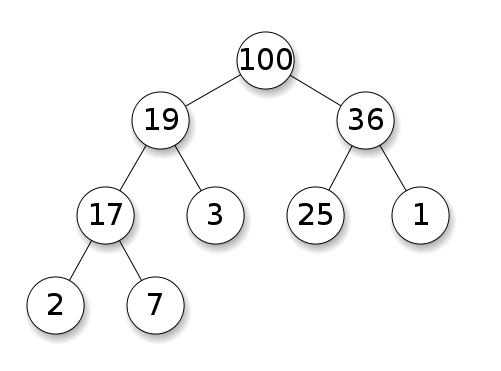
\includegraphics[width=8cm]{./heap.png}
\end{center}
Sin embargo, un \emph{heap} puede representarse como un arreglo en donde dado un indice $i$:
\begin{itemize}
        \item{El padre de $i$ tiene el indice $\mathtt{floor}((i-1)/2)$}
        \item{El hijo derecho de $i$ tiene el indice $2*i+1$}
        \item{El hijo izquierdo de $i$ tiene el indice $2*i+2$}
\end{itemize}

\section*{Procedimiento \emph{ShiftDown} (40\%)}
Dado un arreglo cualquiera, es simple convertirlo a un \emph{heap}. El proceso consiste
en recorrer cada uno de sus indices (empezando desde el final) y convertir dicho indice
en un heap. Para ello se define el metodo \texttt{ShiftDown}\cite{HeapSort} de tipo $\mathtt{ShiftDown}\ :
\ \mathtt{int}[\ ]\otimes\mathtt{int}\rightarrow\mathtt{void}$. El primer parametro es un
arreglo y el segundo parametro es la posici\'on siendo considerada. Este metodo debe hacer
lo siguiente:
\begin{enumerate}
        \item{Se define el indice actual ($i$), el cual se inicializa con el segundo parametro del metodo.}
        \item{Dado el valor ubicado en $i$ y su hijo derecho e izquierdo, seleccionar el valor m\'as peque\~no
        de los tres. Ignorar valores que esten fuera del arreglo. }
        \item{Si el valor seleccionado en el paso anterior es diferente del valor ubicado en $i$,
        intercambiar dicho valor con el valor ubicado en $i$.}
        \item{Si los valores fueron intercambiados, se le asigna a $i$ el indice del valor que fue
        intercambiado y se repite el procedimiento. De lo contrario, el metodo finaliza.}
\end{enumerate}

\section*{Procedimiento \emph{Heapify} (30\%)}
Definir un procedimiento llamado \texttt{Heapify}\cite{HeapSort} de tipo $\mathtt{Heapify}\ :\ \mathtt{int}[\ ]
\rightarrow \mathtt{void}$ el cual recibe un arreglo y lo convierte a su representaci\'on como
\emph{heap}. El procedimiento debe hacer lo siguiente:
\begin{enumerate}
        \item{Comenzar seleccionando el indice ($i$) del padre del ultimo valor en el arreglo (\texttt{Length-1})}
        \item{Llamar al metodo \texttt{ShiftDown} con el arreglo y el indice $i$}
        \item{Decrementar el indice $i$ una unidad}
        \item{Repetir hasta que $i=0$}
\end{enumerate}

\section*{Unit test para \emph{Heapify} (30\%)}
Crear un unit test para el procedimiento \texttt{Heapify}. Este test debe empezar con
un arreglo desordenado, utilizar el metodo \texttt{Heapify} para convertirlo en un \emph{heap}
y por ultimo verifiar que dicho arreglo es un \emph{heap}.

\bibliography{../../Referencias/referencias}
\bibliographystyle{plain}

\end{document}